%\pdfoutput1
%\pdfmapfile{yh.map}
\documentclass[10pt,hyperref={pdfpagelabels=false}]{beamer}

%%%%%%%%%%%%%%%%%% the colors can be changed in next line of codes by passing the correct RGB values %%%%%%%%%%%%%%%%%%%%%%%%%%%%%
\definecolor{kugreen}{RGB}{0,0,56}
\definecolor{kugreenlys}{RGB}{86,157,160}
\definecolor{kugreenlyslys}{RGB}{165,165,165}
\definecolor{kugreenlyslyslys}{RGB}{242,242,242}
\setbeamercovered{transparent}
\setbeamertemplate{caption}[numbered]
\mode<presentation>
{  \usetheme{PaloAlto}
  %\usecolortheme[named=kugreen]{structure}
  \usecolortheme{seahorse}
  \useinnertheme{circles}
  \usefonttheme[onlymath]{serif}
  \setbeamercovered{transparent}
  \setbeamertemplate{blocks}[rounded][shadow=true]
}
\makeatletter
\newcommand\insertlogoii{}
\newcommand\logoii[1]{\renewcommand\insertlogoii{#1}}
\setbeamertemplate{headline}
  {%
    \begin{beamercolorbox}[wd=\paperwidth]{frametitle}
      \ifx\beamer@sidebarside\beamer@lefttext%
      \else%
        \hfill%
      \fi%
      \ifdim\beamer@sidebarwidth>0pt%  
        \usebeamercolor[bg]{logo}%
        \vrule width\beamer@sidebarwidth height \beamer@headheight%
        \hskip-\beamer@sidebarwidth%
        \hbox to \beamer@sidebarwidth{\hss\vbox to
          \beamer@headheight{\vss\hbox{\color{fg}\insertlogo}\vss}\hss}%
        \hfill%
        \vrule width\beamer@sidebarwidth height \beamer@headheight%
        \hskip-\beamer@sidebarwidth%
        \hbox to \beamer@sidebarwidth{\hss\vbox to
          \beamer@headheight{\vss\hbox{\color{fg}\insertlogoii}\vss}\hss}%
      \else%
        \vrule width0pt height \beamer@headheight%  
      \fi%
    \end{beamercolorbox}
}
\makeatother
%\pdfmapfile{/hom/yannis/projets/smf/0/smfpdftex.map}
\usepackage[T1]{fontenc}
\usepackage{amsthm,amsmath,amssymb,amstext,mathtools}
\usepackage[english]{babel}
% \frenchbsetup{og=«,fg=»,AutoSpacePunctuation=false,PartNameFull=true}
%\usepackage{serapion}
\renewcommand{\rmdefault}{cmr}
%\renewcommand{\sfdefault}{univebeamer}
%\renewcommand{\rmdefault}{mtcolumbus}
%\renewcommand{\sfdefault}{mtcolumbus}
\renewcommand{\sfdefault}{syntax}%univebeamer}
\def\textsc#1{{\fontfamily{caeciliasc}\selectfont#1}}
\def\emph#1{{\fontfamily{univebeamer}\selectfont\itshape#1}}
\usepackage{graphics,array,tikz,ifthen,qtree,calc,eurosym,multicol}
%\usetikzlibrary{arrows}
\useoutertheme{sidebar}
\setbeamertemplate{footline}[frame number]
\setbeamertemplate{note page}[plain]
% The following code is partly adapted from code from the alltt package.
\definecolor{lightgreen}{rgb}{.8,1,.9}
\definecolor{mygreen}{RGB}{56,101,103}
\def\sample#1{\textcolor{mygreen}{#1}}

\long\def\smalltexttt#1{{{\fontfamily{fts}\fontsize{9}{10}\selectfont#1

}}}
\long\def\smallertexttt#1{{{\fontfamily{fts}\fontsize{9}{10}\selectfont#1

}}}
\long\def\smallesttexttt#1{{{\fontfamily{fts}\fontsize{8}{9}\selectfont#1

}}}
\def\dotexttt{\fontfamily{fts}\fontsize{\myfontsize}{\mybaselineskip}\selectfont}
\def\dosmalltexttt{\fontfamily{fts}\fontsize{9}{10}\selectfont}
\def\dosmallertexttt{\fontfamily{fts}\fontsize{9}{10}\selectfont}
\def\dosmallesttexttt{\fontfamily{fts}\fontsize{8}{9}\selectfont}

\def\GREEK#1{{\fontencoding{OT1}\fontfamily{mtgrtimes}\fontseries{r}\selectfont#1}} %%%TimesGreSFLiv
\def\ARABIC#1{{\fontencoding{T1}\fontfamily{lemonde}\fontseries{r}\fontshape{arab}\selectfont#1}} %%%NASK1___ h kalutera MyArabic
\def\ajout#1{{\fontencoding{T1}\fontfamily{lemonde}\fontseries{aj}\selectfont#1}} %%%LeMonLivAjo
\def\ajoutbis#1{{\fontencoding{T1}\fontfamily{lemonde}\fontseries{ajt}\selectfont#1}} %%%LeMonLivAjoTwo
\def\down#1{\ensuremath{{}_{\text{#1}}}}
\def\esc#1{\sverb{\\#1}}

\newlength{\loversetlength}
\newlength{\equalsignlength}
\def\loverset#1#2{\settowidth{\equalsignlength}{\ensuremath{=}}\settowidth{\loversetlength}{\ensuremath{#1}}\addtolength{\loversetlength}{-\equalsignlength}\kern-.3\loversetlength\overset{\kern-.1\loversetlength#1}{#2}}

\long\def\mypart#1#2{\begin{frame}{}

\vfill

\Huge\centering#1

\bigskip

\large#2

\vfill\end{frame}}
\setbeameroption{show notes}
\AtBeginNote{\footnotesize\color{black}}
\AtEndNote{\par\hrulefill\par}

\long\def\Kquatre#1#2#3#4#5#6{\begin{tikzpicture}
\tikzstyle{every node}=[draw]
\begin{scope}[shape=circle,minimum size=.1mm]
\node (1) at (0,0) {};
\node (2) at (.8,0) {};
\node (3) at (0,.8) {};
\node (4) at (.8,.8) {};
\end{scope}
\draw[line width=#1] (1) -- (2);
\draw[line width=#2] (1) -- (4);
\draw[line width=#3] (1) -- (3);
\draw[line width=#4] (2) -- (4);
\draw[line width=#5] (3) -- (4);
\draw[line width=#6] (3) -- (2);
\end{tikzpicture}}

\newenvironment{zframe}[1]{\begin{frame}{\rlap{\leavevmode\kern-2.05cm\smash{\raise-8cm\hbox{\resizebox{1.5cm}{!}{\includegraphics{/hom/yannis/texmf/cours/0/Moose-warning.pdf}}}}}#1}}{\end{frame}}

%\font\challEB=ChallExtBolPla at 12pt
%\font\challB=ChallBolPla at 12pt
%\font\textile=Textile at 8pt
%\font\textileB=TextileBol at 9pt
%\def\elem#1{{\fontfamily{textile}\fontseries{bx}\selectfont#1}}
%\def\attr#1{{\fontfamily{textile}\fontseries{m}\selectfont#1}}
\def\inde{\leavevmode\hbox to12pt{}}
\def\retrecipeu#1{\scalebox{.975}[1.0]{$\displaystyle#1$}}
\def\retreci#1{\scalebox{.95}[1.0]{$\displaystyle#1$}}
\def\retrecihalf#1{\scalebox{.925}[1.0]{$\displaystyle#1$}}
\def\retrecii#1{\scalebox{.90}[1.0]{$\displaystyle#1$}}
\def\retreciii#1{\scalebox{.85}[1.0]{$\displaystyle#1$}}
\def\retreciv#1{\scalebox{.80}[1.0]{$\displaystyle#1$}}
\def\retrecitw#1{\resizebox{\textwidth}{\height}{$\displaystyle#1$}}
\def\retreciitw#1{\resizebox{.9\textwidth}{\height}{$\displaystyle#1$}}
\def\retreciiitw#1{\resizebox{.8\textwidth}{\height}{$\displaystyle#1$}}
\def\retrecix#1#2{\resizebox{#1}{\height}{$\displaystyle#2$}}
\def\retreciscale#1#2{\scalebox{#1}[1.0]{$\displaystyle#2$}}
\def\retreciscript#1#2{\scalebox{#1}[1.0]{$\scriptstyle#2$}}
\def\retrecitext#1{\scalebox{.95}[1.0]{$\textstyle#1$}}
\def\retreciitext#1{\scalebox{.90}[1.0]{$\textstyle#1$}}

\def\GREEKb#1{{\fontencoding{OT1}\fontfamily{mtgrtimes}\fontseries{br}\selectfont#1}}
\def\greekbold#1{\ensuremath{\text{\GREEKb{#1}}}}
% ALFABHTO:
% a b g d e z h q i k l m n x o p r s (v) t u f c y w
% Prosochi sta: q = theta, v = sigma teliko, c = chi, y = psi

\let\from\leftarrow
\def\etal{\textit{et al.}}
\SetSymbolFont{operators}{normal}{OT1}{cmr} {m}{n}
\SetSymbolFont{letters}  {normal}{OML}{cmm} {m}{it}
\SetSymbolFont{symbols}  {normal}{OMS}{cmsy}{m}{n}
\def\dingbat#1{{\fontencoding{T1}\fontfamily{lemonde}\fontseries{r}\fontshape{db}\selectfont\char'#1}}
\def\lamain{\leavevmode{\smash{\raise-1.5ex\hbox{\LARGE\dingbat{053}}}}}
\def\TERASTIO#1{{\fontsize{128}{128}\selectfont#1}}
\def\cphantom#1#2{\parbox[c]{\widthof{#1}}{\hss#2\hss}}
\def\textul#1{\ensuremath{\underline{\text{#1}}}}
\DeclareMathOperator*{\argmax}{argmax}
%\catcode`\@=11
%\input{fontmath.ltx}

%\usepackage{mathptmx}
\usepackage{pgflibraryshapes}
\def\mA{\ensuremath{\mathcal{A}}}
\def\mB{\ensuremath{\mathcal{B}}}
\def\mC{\ensuremath{\mathcal{C}}}
\def\mD{\ensuremath{\mathcal{D}}}
\def\mE{\ensuremath{\mathcal{E}}}
\def\mF{\ensuremath{\mathcal{F}}}
\def\mG{\ensuremath{\mathcal{G}}}
\def\mH{\ensuremath{\mathcal{H}}}
\def\mI{\ensuremath{\mathcal{I}}}
\def\mJ{\ensuremath{\mathcal{J}}}
\def\mK{\ensuremath{\mathcal{K}}}
\def\mL{\ensuremath{\mathcal{L}}}
\def\mM{\ensuremath{\mathcal{M}}}
\def\mN{\ensuremath{\mathcal{N}}}
\def\mO{\ensuremath{\mathcal{O}}}
\def\mP{\ensuremath{\mathcal{P}}}
\def\mQ{\ensuremath{\mathcal{Q}}}
\def\mR{\ensuremath{\mathcal{R}}}
\def\mS{\ensuremath{\mathcal{S}}}
\def\mT{\ensuremath{\mathcal{T}}}
\def\mU{\ensuremath{\mathcal{U}}}
\def\mV{\ensuremath{\mathcal{V}}}
\def\mW{\ensuremath{\mathcal{W}}}
\def\mX{\ensuremath{\mathcal{X}}}
\def\mY{\ensuremath{\mathcal{Y}}}
\def\mZ{\ensuremath{\mathcal{Z}}}

\def\bA{\ensuremath{\mathbf{A}}}
\def\bB{\ensuremath{\mathbf{B}}}
\def\bC{\ensuremath{\mathbf{C}}}
\def\bD{\ensuremath{\mathbf{D}}}
\def\bE{\ensuremath{\mathbf{E}}}
\def\bF{\ensuremath{\mathbf{F}}}
\def\bG{\ensuremath{\mathbf{G}}}
\def\bH{\ensuremath{\mathbf{H}}}
\def\bI{\ensuremath{\mathbf{I}}}
\def\bJ{\ensuremath{\mathbf{J}}}
\def\bK{\ensuremath{\mathbf{K}}}
\def\bL{\ensuremath{\mathbf{L}}}
\def\bM{\ensuremath{\mathbf{M}}}
\def\bN{\ensuremath{\mathbf{N}}}
\def\bO{\ensuremath{\mathbf{O}}}
\def\bP{\ensuremath{\mathbf{P}}}
\def\bQ{\ensuremath{\mathbf{Q}}}
\def\bR{\ensuremath{\mathbf{R}}}
\def\bS{\ensuremath{\mathbf{S}}}
\def\bT{\ensuremath{\mathbf{T}}}
\def\bU{\ensuremath{\mathbf{U}}}
\def\bV{\ensuremath{\mathbf{V}}}
\def\bW{\ensuremath{\mathbf{W}}}
\def\bX{\ensuremath{\mathbf{X}}}
\def\bY{\ensuremath{\mathbf{Y}}}
\def\bZ{\ensuremath{\mathbf{Z}}}
\def\cov{\mathrm{cov}}
\usepackage{eurosym}
\let\oldeuro\euro
\def\euro{\ensuremath{\text{\oldeuro}}}

\newcommand{\bigmaltese}{%
  \mathop{ % we want it to be an operator
    \mathchoice{\dobigmaltese\Large}
               {\dobigmaltese\large}
               {\dobigmaltese\normalsize}
               {\dobigmaltese\small}
    }\displaylimits % not necessary, but added for clarity
}

\newcommand{\dobigmaltese}[1]{%
  \vcenter{#1\kern.2ex\hbox{$\maltese$}\kern.2ex}}

\def\intervalleoo#1{\mathopen{]}#1\mathclose{[}}
\def\intervallefo#1{\mathopen{[}#1\mathclose{[}}
\def\intervalleof#1{\mathopen{]}#1\mathclose{]}}
\def\transpose#1{{}^t#1}
\endinput

\def\sverb#1{\texttt{{\color{black}\def\\{\textbackslash}#1}}}
\let\oldemph=\emph
\def\emph#1{{\color[rgb]{0,0,1}\oldemph{#1}}}
\def\defi#1{{\color{blue}#1}}
\renewcommand{\defi}[2][nil]{{\color{blue}#2}}
\logo{
\includegraphics[width=35pt]{VJTIM.jpg}}
%\rlap{\includegraphics[width=45pt,viewport=100 506.5 200 506.5]{by-nc-nd-eu.pdf}}}
\def\Attention{\framebox{\color{blue}\textsc{Attention !}}}
\def\bellepage{}

{\catcode`\^^M=13 % these lines must end with %
  \gdef\obeylines{\catcode`\^^M=13 \let^^M\par}%
  \global\let^^M\par}

\catcode`\@=11
\begingroup
\lccode`\~=`\'
\lowercase{\endgroup
\renewenvironment{semiverbatim}{%
  \color{black}\trivlist
  \item\relax
    \if@minipage
    \else
      \vskip\parskip
    \fi
    \leftskip\@totalleftmargin
    \rightskip\z@skip
    \parindent\z@
    \parfillskip\@flushglue
    \parskip\z@skip
    \@@par
    \@tempswafalse
    \def\par{%
      \if@tempswa
        \leavevmode\null\@@par\penalty\interlinepenalty
    \else
      \@tempswatrue
      \ifhmode\@@par\penalty\interlinepenalty\fi
    \fi}
    \obeylines
    \def\verbatim@nolig@list{\do\`\do\,\do\'\do\-}
    \verbatim@font
    \let\org@prime~%
    \everymath\expandafter{\the\everymath
      \catcode`\'=12 \let~\org@prime}
    \everydisplay\expandafter{\the\everydisplay
      \catcode`\'=12 \let~\org@prime}
    \def\dospecials{\do\ \do\$\do\&%
     \do\#\do\^\do\_\do\%\do\~\do\`\do\,\do\'\do\-}
    \let\do\@makeother
    \dospecials
    \def\\{\char`\\}
    \def\{{\char`\{}
    \def\}{\char`\}}
    \frenchspacing\@vobeyspaces
    \everypar \expandafter{\the\everypar \unpenalty}}
{\endtrivlist}}

\let\utemize\itemize
\let\endutemize\enditemize
\let\utem\item
\let\usection\section
\let\usubsection\subsection
\def\usubsubsection#1{}
\let\niv\quad

%\long\def\note#1{#1}
\long\def\pres#1{#1}
\long\def\poly#1{}
%\let\usection\chapter

\newtheorem{prop}{Proposition}[section]
\newtheorem{theo}[prop]{Theorem}
\newtheorem{lemm}[prop]{Lemma}
\newtheorem{coro}[prop]{Corollary}
\newtheorem{defien}[prop]{Definition}
\newtheorem{defis}[prop]{Definitions}

\def\WHITEFRAME{\bgroup
\setbeamercolor{background canvas}{bg=white}
\setbeamertemplate{navigation symbols}{}
\begin{frame}[plain]{}
\end{frame}
\egroup}
\def\RAPPEL{\setbeamercolor{normal text}{fg=black,bg=black!40}

\setbeamercolor{structure}{fg=black}

\setbeamercolor{alerted text}{fg=red!85!black}

\setbeamercolor{item projected}{use=item,fg=black,bg=item.fg!75}

\definecolor{beetle@other}{RGB}{64,80,127}

\setbeamercolor*{palette primary}{fg=white,bg=beetle@other}
\setbeamercolor*{palette secondary}{parent=palette primary,use=palette primary,bg=palette primary.bg!95!black}
\setbeamercolor*{palette tertiary}{parent=palette primary,use=palette primary,bg=palette primary.bg!90!black}
\setbeamercolor*{palette quaternary}{parent=palette primary,use=palette primary,bg=palette primary.bg!85!black}

\setbeamercolor*{sidebar}{parent=palette primary}

\setbeamercolor*{palette sidebar primary}{fg=white}
\setbeamercolor*{palette sidebar secondary}{fg=black}
\setbeamercolor*{palette sidebar tertiary}{fg=white}
\setbeamercolor*{palette sidebar quaternary}{fg=black}

\setbeamercolor{framesubtitle}{fg=black}

\setbeamercolor*{subtitle}{fg=black}

\setbeamercolor*{block title}{parent=structure}
\setbeamercolor*{block title alerted}{parent=alerted text}
\setbeamercolor*{block title example}{parent=example text}
\setbeamercolor*{block body}{}
\setbeamercolor*{block body alerted}{}
\setbeamercolor*{block body example}{}

\setbeamercolor*{titlelike}{parent=structure}
}
\def\myindex#1{}
\let\shaded\relax
\let\endshaded\relax
\usepackage{mdframed,bussproofs,comment,attachfile}
%\usepackage{thsmc}
\def\partname{Partie}
\newlength{\cleaplengtha}
\newlength{\cleaplengthb}
\def\cphantom#1#2{\settowidth{\cleaplengtha}{#1}%
\settowidth{\cleaplengthb}{#2}\addtolength{\cleaplengthb}{-\cleaplengtha}\leavevmode\hbox{}\kern.5\cleaplengthb#1\kern.5\cleaplengthb\hbox{}}
%\newtheorem{definition}{Définition}
%\newtheorem{definitions}[definition]{Définitions}
\endinput
\usepackage{pgfpages,qtree,url,fontspec,dad}
\usepackage{media9}
\usepackage[font=scriptsize]{caption}
%\usepackage[utf8x]{inputenc}
\setbeameroption{hide notes}
\usepackage{tikz-dependency}
\usepackage[round]{natbib}
\renewcommand{\newblock}{}
%\usepackage[all]{xy}
\newcounter{saveenumi}
\newcommand{\seti}{\setcounter{saveenumi}{\value{enumi}}}
\newcommand{\conti}{\setcounter{enumi}{\value{saveenumi}}}
\usepackage{amsmath,amsfonts,amscd,multicol,eurosym,array,yhmath}
\usepackage{bm}% bold math
\usepackage{ragged2e}
\usepackage{multirow}

\newcommand{\mathcolorbox}[2]{\colorbox{#1}{$\displaystyle #2$}}
%\def\rmdefault{cmr}
%\def\sfdefault{cmr}
%\usepackage{ucs}
%\usepackage[utf8]{inputenc}
%\usepackage[T1]{fontenc}
%\usepackage[francais]{babel}

%%%%%%%%%%%%%%%%%%%%%%%%%%%%%%%%%%%%%%%%%%%%%%%
%% ADD Title Here

\title{APS II:\\
Gaussian Process Surrogate Model for an Effective Life Assessment of Transformer}

%%%%%%%%%%%%%%%%%%%%%%%%%%%%%%%%%%%%%%%%%%%%%%%
%% ADD Author name here 

\author{Shadab Nayyer}
\institute{ID: 199030002\\Research Scholar\\  CDRC, EED, VJTI, Mumbai \\\vspace{2mm}
Supervisor(s): Dr. N. M. Singh\\
\hspace{15.5mm}Dr. S. R. Wagh}


%\author{Pooja Kamlakar Waghmode}
%\institute[Veermata Jijabai Technological Institute, Mumbai]{ ID: 192071022\\
%M.Tech EED(Control System) \\
%\vspace{2mm}
%Supervisor: Dr. N M Singh\\
%\hspace{19mm}Dr. Sushma Wagh
%}
\date{\today}
\logo{
\includegraphics[height=1.5cm]{VJTIM.jpg}}
\logoii{
\includegraphics[height=1.2cm]{CDRC_Logo.jpeg}}


\begin{document}
%\fontfamily{cmr}\selectfont
\maketitle
\def\yem#1{\texttt{\textbackslash #1} $\csname#1\endcsname$\relax}

%%%%%%%%%%%%%%%%%%%%%%%%%%%%%%%%%%%%%%%%%%%%%%%%%%%%%%%%%%%%%%%%%%
%\section{Contents}
\begin{frame}[fragile]
\frametitle{Contents} 

\tableofcontents
%\item Mindmap
 %   \item System Model of a Smart Building
  %  \item Load Profile Prediction for a smart building using data driven approach
   % \begin{enumerate}
    %    \item Electricity consumption profile prediction for a smart building using polynomial regression
     %   \item Smart building load profile prediction using ANN
       % \item Load profile prediction for a smart building using DMD
        %\item Implementation of GPR for predicting the smart building electricity consumption profile 
    %\end{enumerate}
    %\item Conclusion and Future Work
\end{frame}
%%%%%%%%%%%%%%%%%%%%%%%%%%%%%%%%%%%%%%%%%%%%%%%%%%

\section{Recap: APS-1}
\begin{frame}[fragile]
\frametitle{Recap: APS-1}
    \begin{columns}[c] % The "c" option specifies centered vertical alignment while the "t" option is used for top vertical alignment

\column{.5\textwidth}
\textbf{Inverse Problem}:\\
The physical parameter characterizing a model:
\begin{equation*}
    y=m\hspace{0.1cm}\theta
\end{equation*}
\textbf{The forward problem}: Finding the "y" given $\theta$.

\textbf{The Inverse  problem}: Finding the "$\theta$" given y.
\textbf{Parameter Estimation methods}
\begin{enumerate}
    \item Concurrent learning
    \item Composite learning
    \item DREM
\end{enumerate}
\column{.52\textwidth}

\begin{block}{Example}
A quadratic equation
\begin{equation*}
    y(t)=\theta_1*m_1+\theta_2*m_2 
\end{equation*}
Data points at different time interval, a system equation with p rows and n columns
\begin{equation*}
    \begin{bmatrix}
m_{11} &m_{21} \\ 
m_{12} & m_{22}\\
m_{13} &m_{23}
\end{bmatrix}*\begin{bmatrix}
\theta_1\\ 
\theta_2
\end{bmatrix}=\begin{bmatrix}
y_1\\ 
y_2\\ 
y_3
\end{bmatrix}
\end{equation*}
\begin{equation*}
    \left \| y-m\theta \right \|_2=\sqrt{\sum_{i=1}^{m}(y_i-(m\theta)_i)^2}
\end{equation*}
\end{block}
\end{columns}
\end{frame}
%%%%%%%%%%%%%%%%%%%%%%%%%%%%%%%%%%%%%%%%%%%%%%
\section{Mindmap}
\begin{frame}[fragile]
\frametitle{Objectives and Mindmap}
\begin{figure}
    \centering
    %\includegraphics[width=0.95\textwidth]{Images/PPM.png}
    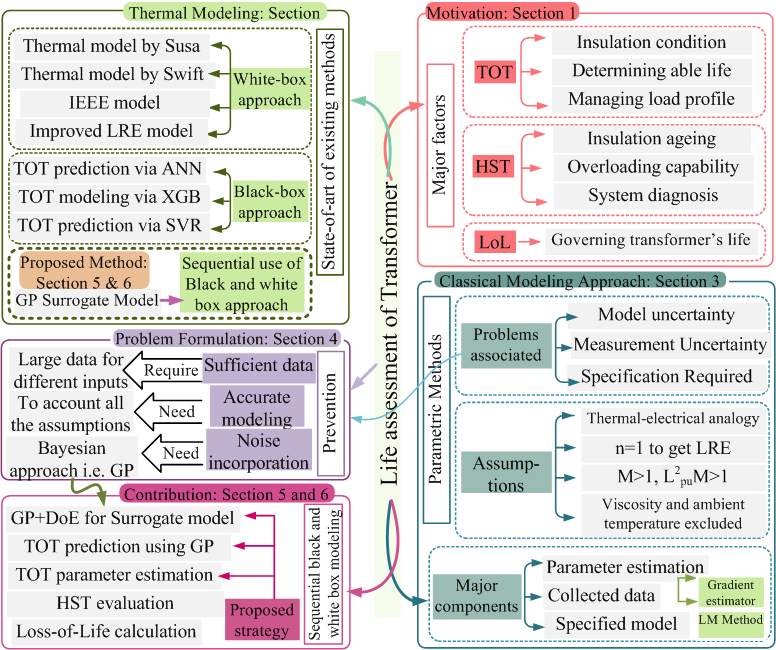
\includegraphics[scale=0.31]{Mindmap_APS_R1.png}
    \caption{Mind map for life assessment of transformer}
   % \label{fig:Problem_5_1_1}
\end{figure}

\end{frame}

%%%%%%%%%%%%%%%%%%%%%%%%%%%%%%%%%%%%%%%%%%%%%%
\section{Classical Modelling Approach}
\begin{frame}[fragile]
\frametitle{Classical Modelling Approach}
The energy-balance equation represented in Fig. 2(a) 
\begin{small}
\begin{align}\label{rcequation}
    \mathrm{q_{FE}}+\mathrm{q_{CU}}=\mathrm{C}_{\mathrm{TH-OIL}}\frac{\mathrm{d} \vartheta_{\mathrm{TOT}}}{\mathrm{d} \mathrm{t}}+
    \frac{(\vartheta_{\mathrm{TOT}}-\vartheta_{\mathrm{AMB}})}{\mathrm{R}_{\mathrm{TH-OIL}}}
\end{align}
\end{small}
\begin{small}
\begin{equation}\label{s1}
    \frac{1+\mathrm{M} \mathrm{L}_{\mathrm{pu}}^2}{1+\mathrm{M}}  \nu_{\mathrm{pu}}^{\boldsymbol{\mathfrak{n}}}  \Delta\vartheta_{\mathrm{TOTR}}=
    \nu_{\mathrm{pu}}^{\boldsymbol{\mathfrak{n}}} \Gamma_{\mathrm{TOTR}}\frac{\mathrm{d} \vartheta_{\mathrm{TOT}}}{\mathrm{d} \mathrm{t}}+\frac{\left ( \vartheta_{\mathrm{TOT}}-\vartheta_{\mathrm{AMB}} \right )^{1+{\boldsymbol{\mathfrak{n}}}}}{(\Delta\vartheta_{\mathrm{TOTR}})^{\boldsymbol{\mathfrak{n}}}}.
\end{equation}
 \end{small}
\begin{figure}
    \centering
    %\includegraphics[width=0.95\textwidth]{Images/PPM.png}
    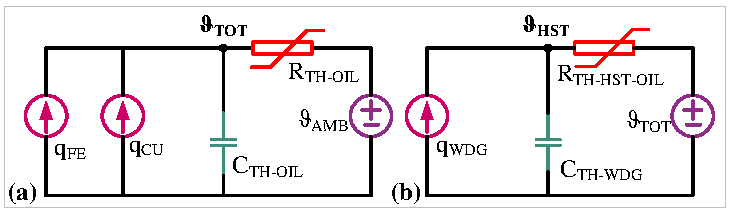
\includegraphics[scale=0.70]{Images/RC11.pdf}
    \caption{Thermal circuits: (a) TOT model (b) HST model}
    \label{fig:Problem_5_1_1}
\end{figure}
\begin{small}
\begin{equation}\label{hs1}
     \mathrm{P}_{\mathrm{WDG,pu}}(\vartheta_{\mathrm{HST}})\times \mathrm{L}_{\mathrm{pu}}^2  \nu_{\mathrm{pu}}^{\boldsymbol{\mathfrak{n}}} \Delta\vartheta_{\mathrm{HSTR}}=
\nu_{\mathrm{pu}}^{\boldsymbol{\mathfrak{n}}} \Gamma_{\mathrm{WDGR}}\frac{\mathrm{d} \vartheta_{{\mathrm{HST}}}}{\mathrm{d} \mathrm{t}}+\frac{\left ( \vartheta_{\mathrm{HST}}-\vartheta_{\mathrm{TOT}} \right )^{1+{\boldsymbol{\mathfrak{n}}}}}{(\Delta\vartheta_{{\mathrm{HSTR}}})^{\boldsymbol{\mathfrak{n}}}}
\end{equation}
\end{small}
\end{frame}

%%%%%%%%%%%%%%%%%%%%%%%%%%%%%%%%%%%%%%%%%%%%%%
%%%%%%%%%%%%%%%%%%%%%%%%%%%%%%%%%%%%%%%%%%%%%%
\section{Limitations of Classical Modelling}
\begin{frame}[fragile]
\frametitle{Limitations of Classical Modelling}

\begin{columns}
\column{0.50\textwidth}
\begin{block}{Measurement Uncertainty}
\scriptsize
\begin{enumerate}
    \item The thermal models are developed in \cite{susa} and \cite{swift} using the thermal-electrical analogy.
    %
    \item When $\mathrm{M}>1$ and $\mathrm{L}_{\mathrm{pu}}^2 \mathrm{M}>1$, the $\vartheta_{\mathrm{ULT}}$ can be approximate to $\Delta \vartheta_{\mathrm{\mathrm{TOTR}}} \mathrm{L}_{\mathrm{pu}}^{2{\boldsymbol{\mathfrak{n}}}}$ \cite{lesieutre}.
    %
    \item For natural convection $\boldsymbol{\mathfrak{n}}=0.8$ and for forced cooling $\boldsymbol{\mathfrak{n}}=0.9-1.0$ loading guide \cite{Pierce}. To get LRE for simplification  \cite{lesieutre}, $\boldsymbol{\mathfrak{n}}=1$.
\end{enumerate}
\end{block}
\begin{alertblock}{Measurement Uncertainty}
\scriptsize
    It is highly possible that the data collected may get corrupted due to sensor-noise and environmental conditions. The data with noise introduces measurement uncertainty and affects the thermal model's accuracy, HST, and LoL calculation. 
\end{alertblock}
\column{0.45\textwidth}
\begin{alertblock}{Specifications required}
\scriptsize
The $\Gamma_{\mathrm{WDGR}}$, and $\Delta\vartheta_{\mathrm{HSTR}}$ are based on\\ $\mathrm{R}_{\mathrm{TH-HST-OILR}}= \mathrm{R}_{\mathrm{TH-OILR}}$.\\
The rated nonlinear thermal resistance with \\$\nu=\nu_{pu} \times \nu_R$ is 
 %\begin{equation}\label{ RTHOILR}
   $\mathrm{R}_{\mathrm{TH-OILR}}=\frac{1}{C_1A} \times \left ( \frac{\nu_R }{\Delta\vartheta_{\mathrm{TOTR}}}\right )^{\boldsymbol{\mathfrak{n}}}$,\\
 %\end{equation}

% \begin{equation}\label{deltatheta}
    $ \Delta \vartheta_{\mathrm{TOTR}}=(\mathrm{q}_{\mathrm{FE}}+\mathrm{q}_{\mathrm{CU}})_R\times \mathrm{R}_{\mathrm{TH-OILR}}$, 
% \end{equation}
 and 
% \begin{equation}\label{toil}
 $\Gamma_{\mathrm{TOTR}}=\mathrm{R}_{\mathrm{TH-OILR}} \times \mathrm{C}_{\mathrm{TH-OILR}}$\\
 %\end{equation}
are the constant parameters. Calculation of which requires area $A$, a constant $C_1$, $q_{\mathrm{FE}}$, $q_{\mathrm{CU}}$, supplied losses and $\nu_\mathrm{R}$ for these parameter determination.


\end{alertblock}
\begin{exampleblock}{\textbf{Remark:}}
\scriptsize
Practically, it is possible that the complete specification of transformer might not be readily available or improper values may lead to the erroneous calculations.
\end{exampleblock}
\end{columns}



\end{frame}

%%%%%%%%%%%%%%%%%%%%%%%%%%%%%%%%%%%%%%%%%%%%%%
%%%%%%%%%%%%%%%%%%%%%%%%%%%%%%%%%%%%%%%%%%%%%%
%\section{Classical Modelling Approach}
\begin{frame}[fragile]
\frametitle{Limitations of the parametric approaches  (Polynomial Regression and Neural Network)}
\begin{figure}
    \centering
    %\includegraphics[width=0.95\textwidth]{Images/PPM.png}
    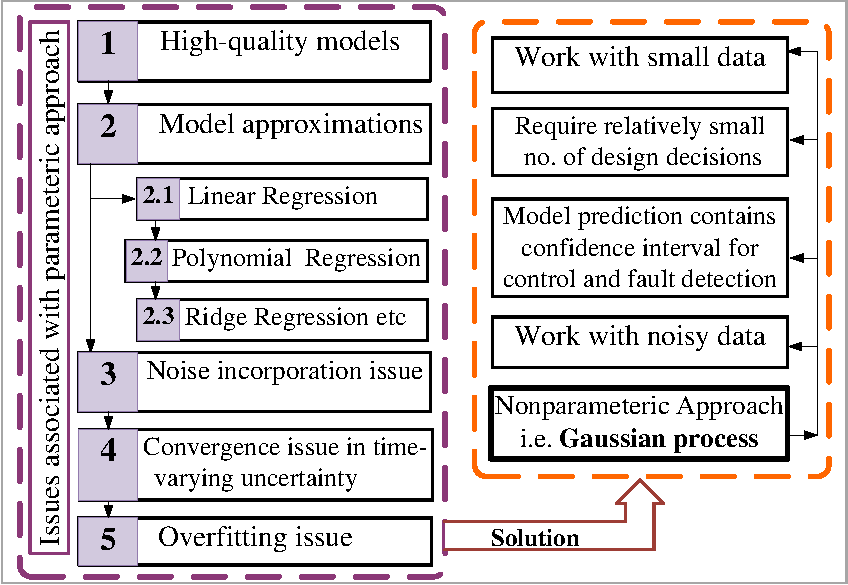
\includegraphics[scale=0.6]{Images/pdfresizer.com-pdf-crop (12).pdf}
    \caption{Issues with classical regression and its solution is given by GP}
    \label{fig:Problem_5_1_1}
\end{figure}

\end{frame}
%%%%%%%%%%%%%%%%%%%%%%%%%%%%%%%%%%%%%%%%%
\section{Gaussian Process}
\begin{frame}[fragile]
\frametitle{Gaussian Process}
\begin{columns}
\column{0.55\textwidth}
A TOT thermal model
\begin{equation}\label{e7}
   y=\eta(\mathrm{x})+\delta 
\end{equation}
The data $\left [ y_1,\dots,y_n \right ]^T\sim \mathcal{GP}(0, \mathbb{K})$ with 
\begin{equation}\label{e8}
    \mathbb{K}=\Sigma_{\eta}+\delta_{\delta}^2I
\end{equation}
The elements of $\Sigma_{\eta}$ 
 \begin{equation*}\label{e4}
     \Sigma_{ij}=cov(\eta(\mathrm{x}_{i}), \eta(\mathrm{x}_{j}))=\mathbb{C}(\mathrm{x}_i,\mathrm{x}_j)
 \end{equation*}
  and covariance function 
  \begin{small}
 \begin{align*}\label{e6}
     \mathbb{C}(\mathrm{x}_i,\mathrm{x}_j)=\sigma_{\eta}^2\hspace{0.1cm}\\exp\left [ -\frac{1}{2}\sum_{e=1}^{\mathrm{E}}\rho _e(\mathrm{x}_{ie}-\mathrm{x}_{je})^2 \right ]+\sigma_{\delta}^2\delta_{ij}^k
 \end{align*}
  \end{small}
 The mean and covariance of posterior 

\column{0.51\textwidth}

\begin{equation*}\label{e10}
     \mu (\mathrm{x}^*)=E_{\eta}\left ( \eta(\mathrm{x}^*)\mid \mathrm{X}, y, \Theta \right )
\end{equation*}
\begin{equation*}\label{e11}
     \sigma^2(\mathrm{x}^*)=\mathrm{var}_{\eta}\left ( \eta(\mathrm{x}^*)\mid \mathrm{X}, y, \Theta \right )
\end{equation*}
%For the random variable set $\left \{ y_1,\dots,y_n,y^*\right \}$, 
the prediction of $y^*$ is given as
 \begin{equation}\label{e12}
     y, y^* \sim\mathcal{N}(0, \mathbb{K}_{n+1}),
 \end{equation}
with covariance matrix
\begin{equation*}\label{e13}
    \mathbb{K}_{n+1}=\begin{bmatrix}
 \mathbb{K}& k(\mathrm{x}^*)\\ 
k^T(\mathrm{x}^*) & \boldsymbol{K}(\mathrm{x}^*)
\end{bmatrix}.
\end{equation*}
%Predictive distribution with  mean and variance as:
\begin{equation*}\label{e14}
    E(y^*)=\mu(\mathrm{x}^*)=k^T(\mathrm{x}^*)\mathbb{K}^{-1}y
\end{equation*}
\begin{align*}\label{e15}
   \mathrm{ var}(y^*)=\sigma(\mathrm{x}^*)=\\\boldsymbol{K}(\mathrm{x}^*)-k^T(\mathrm{x}^*)\mathbb{K}^{-1}k(\mathrm{x}^*)
\end{align*} 

\end{columns}
\end{frame}
%%%%%%%%%%%%%%%%%%%%%%%%%%%%%%%%%%%%%%%%%%%%%%
\section{Data Driven Surrogate Model}
\begin{frame}[fragile]
\frametitle{GP Surrogate Model}
\begin{figure}
    \centering
    %\includegraphics[width=0.95\textwidth]{Images/PPM.png}
    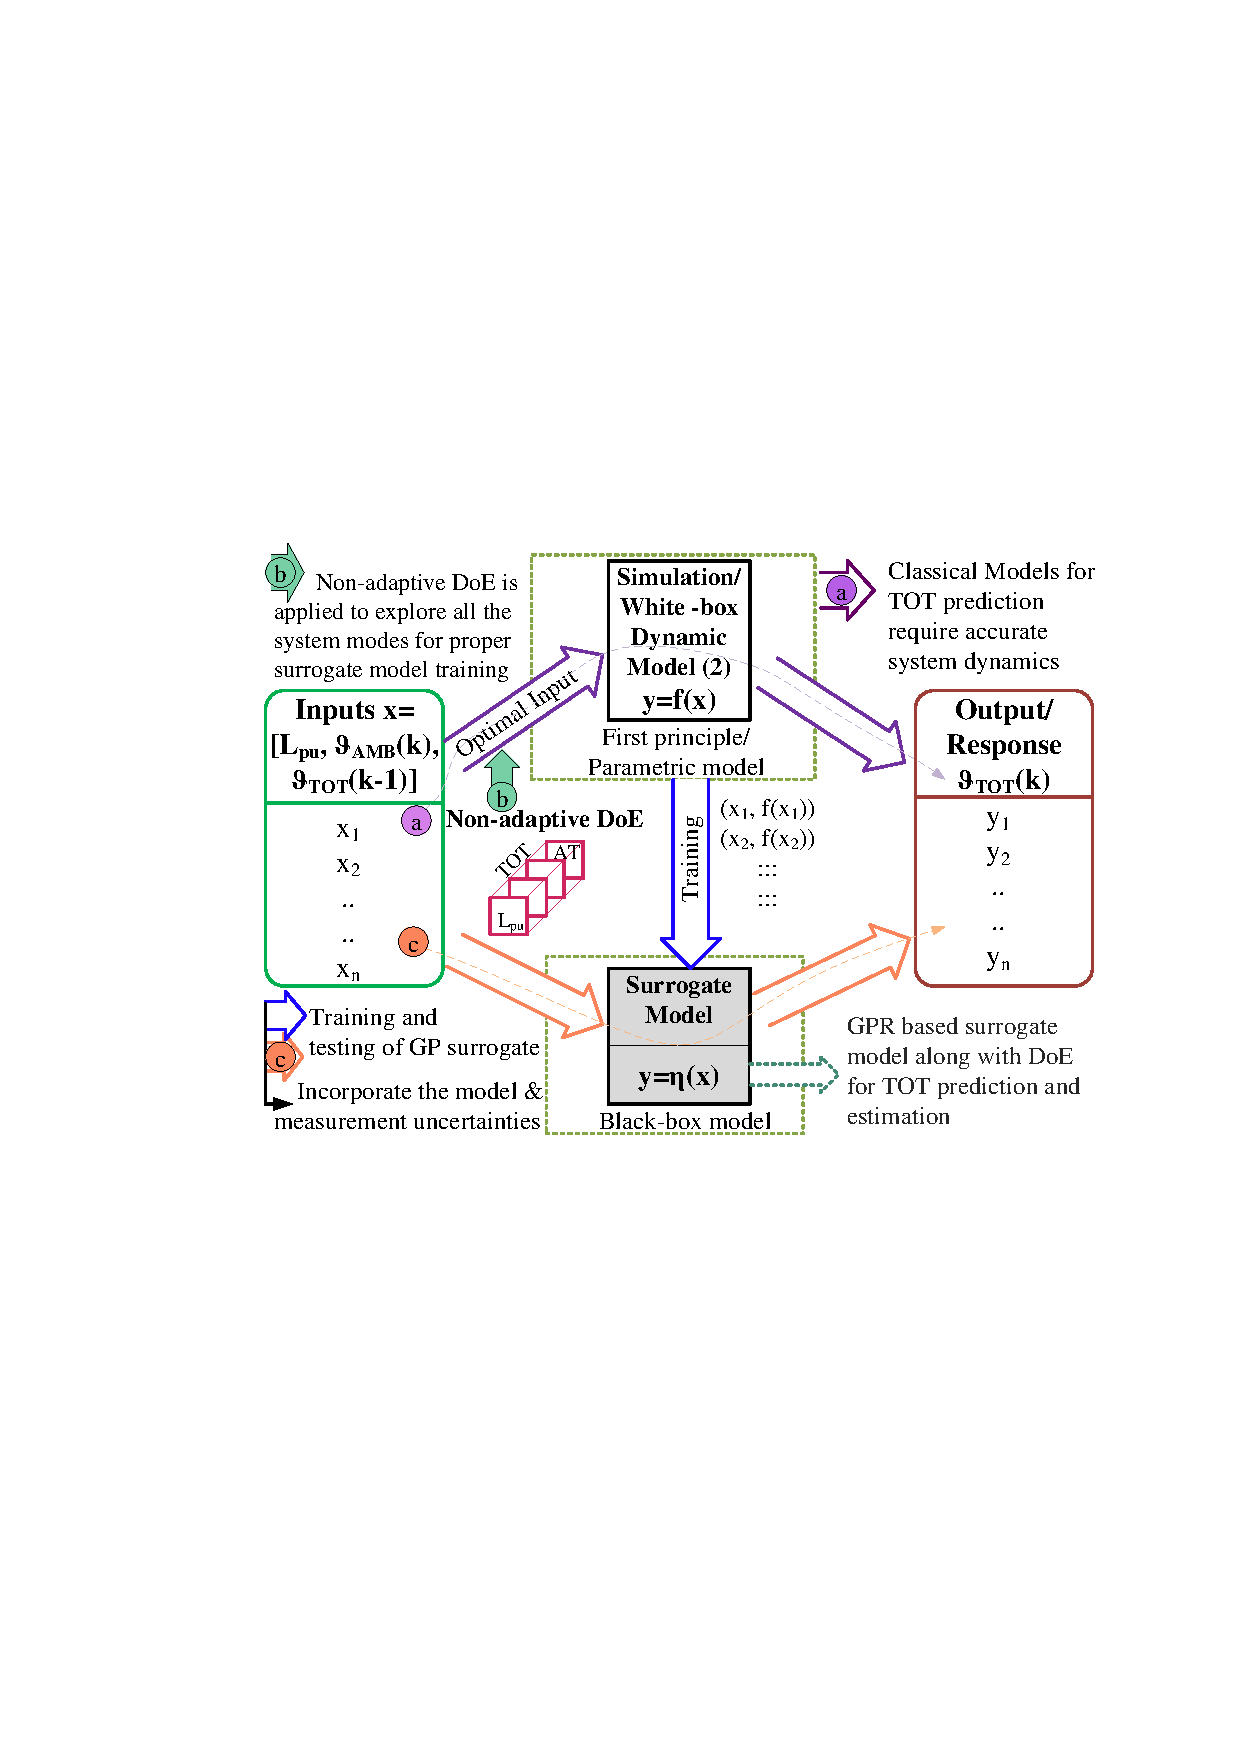
\includegraphics[scale=0.6]{Images/1_updated_TOTO_Pred_Else_r3.pdf}
    \caption{The development of GP surrogate model for TOT prediction. The input-output mappings are shown via dynamic model (purple) and the surrogate model (orange)}
    \label{fig:Problem_5_1_1}
\end{figure}

\end{frame}

%%%%%%%%%%%%%%%%%%%%%%%%%%%%%%%%%%%%%%%%%%%%%%
\section{Transformer Life Assessment}
\begin{frame}[fragile]
\frametitle{Life Assessment of Transformer using \\ SBAWB Modeling}
\begin{columns}
\column{0.53\textwidth}
\begin{alertblock}{TOT Prediction \& Estimation}
\scriptsize
\begin{enumerate}
    \item The quality data of the TOT, AT and loading is generated using DoE and GPR.
    \item The LM algorithm is implemented for estimation problems
\end{enumerate}
\end{alertblock}
\begin{block}{HST Calculation}
\scriptsize
\begin{itemize}
    \item The calculation of $\Delta\vartheta_{\mathrm{HSTR}}$, and $\Gamma_{\mathrm{WDG}}$ need $\mathrm{R}_{\mathrm{TH-OIL}}$.
    \item The $\mathrm{R}_{\mathrm{TH-OIL}}$ is obtained using $\Gamma_{\mathrm{TOT}}$. the parameters ($\Delta\vartheta_{\mathrm{HSTR}}$,  $\Gamma_{\mathrm{WDG}}$), the HST is obtained.
\end{itemize}
\end{block}
\begin{exampleblock}{Loss-of-Life}
\scriptsize
\begin{equation*}
    \mathrm{per\hspace{0.1cm}unit\hspace{0.1cm}life} =\mathbb{A}\hspace{0.1cm}exp\left [ \frac{\beta}{\vartheta_{\mathrm{HST}}+273} \right ]
\end{equation*}
\begin{equation*}
    \mathrm{F}_{\boldsymbol{AA}}=exp\left [ \frac{15000}{383}-\frac{15000}{\vartheta_{\mathrm{HST}}+273} \right ]
\end{equation*}
\end{exampleblock}
\column{0.54\textwidth}

\begin{figure}
    \centering
    %\includegraphics[width=0.95\textwidth]{Images/PPM.png}
    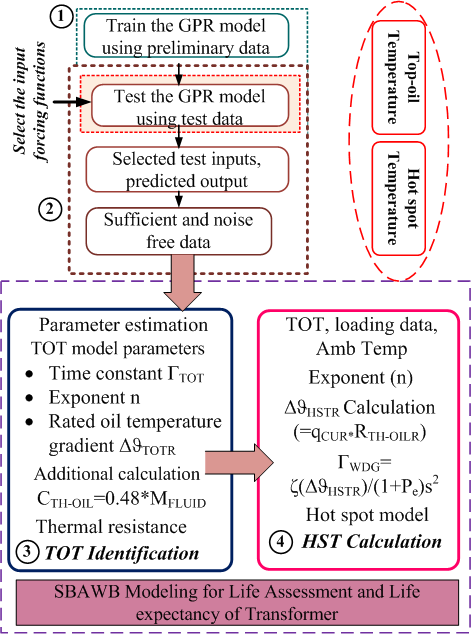
\includegraphics[scale=0.3]{APS_fig11.png}
    %\caption{A systematic procedure of life assessment  using  SBAWB Modeling. }
    \label{fig:Problem_5_1_1}
\end{figure}
\end{columns}
\end{frame}

%%%%%%%%%%%%%%%%%%%%%%%%%%%%%%%%%%%%%%%%%%%%%%
\section{Results}
\begin{frame}[fragile]
\frametitle{Results of SBAWB Modeling for Prediction\\ and Estimation}
\begin{columns}
\column{0.5\textwidth}
\begin{figure}
    \centering
    %\includegraphics[width=0.95\textwidth]{Images/PPM.png}
    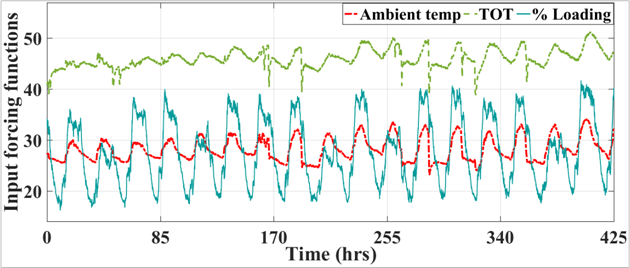
\includegraphics[scale=0.23]{Images/Amb_real_NEW_8Pages_OL.png}
    \caption{Real-time data of the measured TOT, \% loading, and AT}
    \label{fig:Problem_5_1_1}
\end{figure}
\begin{figure}
    \centering
    %\includegraphics[width=0.95\textwidth]{Images/PPM.png}
    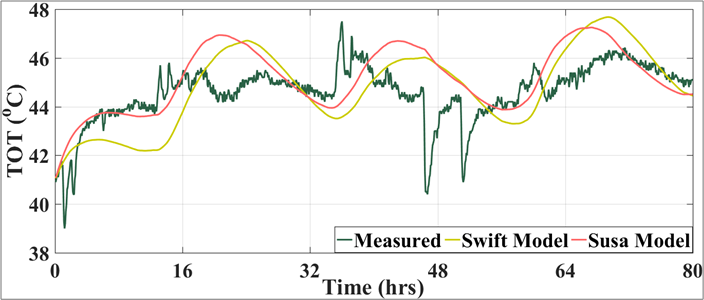
\includegraphics[scale=0.2]{Images/SUSA_SWIFT_comparison_OL.png}
    \caption{Measured and estimated TOT  using parametric models}
    \label{fig:Problem_5_1_1}
\end{figure}
\column{0.5\textwidth}
\begin{figure}
    \centering
    %\includegraphics[width=0.95\textwidth]{Images/PPM.png}
    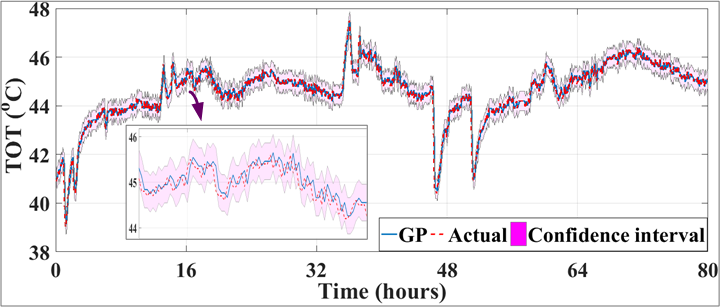
\includegraphics[scale=0.18]{Images/Gp_real-time_1000_OL.png}
    \caption{Measured (red dashed) and predicted (blue solid) TOT using GP.}
    \label{fig:Problem_5_1_1}
\end{figure}
\begin{figure}
    \centering
    %\includegraphics[width=0.95\textwidth]{Images/PPM.png}
    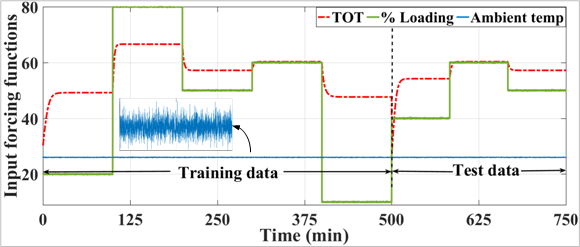
\includegraphics[scale=0.25]{Images/virtual_oil_temp_8Pages_new_OL.png}
    \caption{MATLAB (Virtually generated) data }
    \label{fig:Problem_5_1_1}
\end{figure}
\end{columns}
\end{frame}

%%%%%%%%%%%%%%%%%%%%%%%%%%%%%%%%%%%%%%%%%%%%%%
%%%%%%%%%%%%%%%%%%%%%%%%%%%%%%%%%%%%%%%%%%%%%%
%\section{Results}
\begin{frame}[fragile]
\frametitle{Results of SBAWB Modeling for Prediction\\ and Estimation (cont...)}
\begin{columns}
\column{0.6\textwidth}
\begin{figure}
    \centering
    %\includegraphics[width=0.95\textwidth]{Images/PPM.png}
    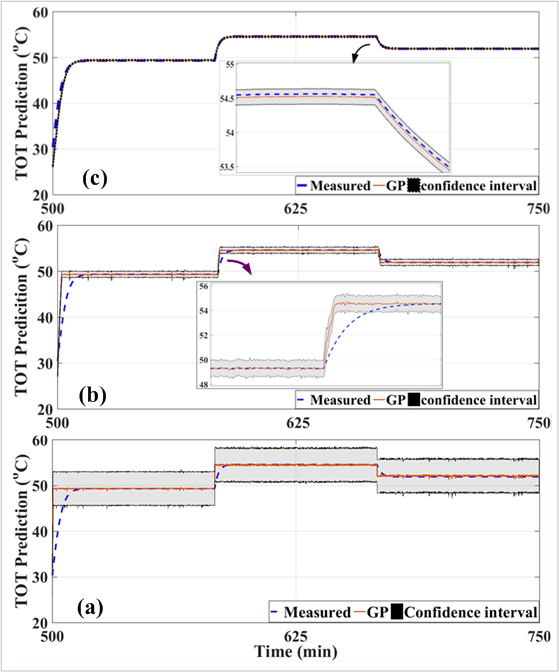
\includegraphics[scale=0.425]{Images/SSN_graphs_CI.png}
    \caption{The TOT prediction using GPR:\\ $(\mathbf{a})$ SNR 5 and 10 dB, \\$(\mathbf{b})$ with SNR 20 and 10 dB\\ $(\mathbf{c})$ without noise.}
    \label{fig:Problem_5_1_1}
\end{figure}
\column{0.45\textwidth}
\begin{figure}
    \centering
    %\includegraphics[width=0.95\textwidth]{Images/PPM.png}
    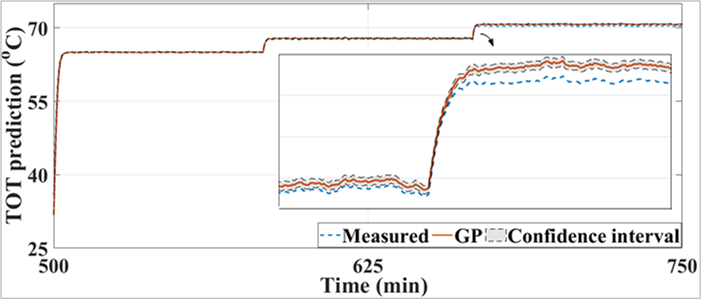
\includegraphics[scale=0.20]{Images/Figure_final_extrapolate_R2.png}
    \caption{The TOT prediction using GP surrogate model for test data  }
    \label{fig:Problem_5_1_1}
\end{figure}
\begin{figure}
    \centering
    %\includegraphics[width=0.95\textwidth]{Images/PPM.png}
    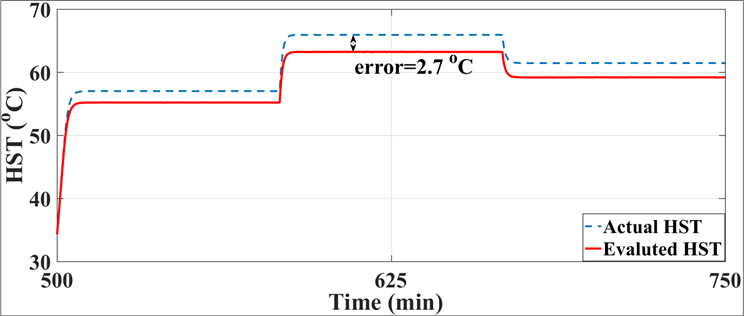
\includegraphics[scale=0.19]{Images/HST_virtual.png}
    \caption{Simulated HST evaluation }
    \label{fig:Problem_5_1_1}
\end{figure}
\column{0.5\textwidth} 
\end{columns}
\end{frame}
%%%%%%%%%%%%%%%%%%%%%%%%%%%%%%%%%%%%%%%%%%%%%%
%\section{Results}
\begin{frame}[fragile]
\frametitle{Error analysis}
\begin{columns}
\column{0.5\textwidth} 
\begin{exampleblock}{Error parameters}
\scriptsize
\begin{equation}
    \mathrm{RMSE}=\sqrt{\frac{1}{n}\sum_{i=1}^{n}(y^{\mathfrak{D}}_i-y_i)^2},
\end{equation}
\begin{equation}
    \mathrm{MAE}=\frac{1}{n}\sum_{i=1}^{n}\left | y^{\mathfrak{D}}_i-y_i \right |,
\end{equation}
\begin{equation*}
    \mathrm{CC}=\frac{\sum_{i=1}^{n}(y^{\mathfrak{D}}_i-\bar{y}^{\mathfrak{D}})(y_i-\bar{y})}{\sqrt{\sum_{i=1}^{n}(y^{\mathfrak{D}}_i-\bar{y}^{\mathfrak{D}})^2\sum_{i=1}^{n}(y_i-\bar{y})^2}}
\end{equation*}
\end{exampleblock}
\begin{alertblock}{Comparison}
\scriptsize
The average RMSE for training data  is $2.03\pm 1.01$ of ANN, $2.37\pm0.77$ of SVR , and  $1.67\pm1.14$ of XGB. The average RMSE for test dataset is 1.9825 of Recurrent Neural Network (RNN),  $5.8$ of ANN, and 2.225 of ARX model is observed in a comparative study. \end{alertblock}
\column{0.5\textwidth} 
\begin{table}[h!]
\caption{Comparison of the different classical models and GP for TOT prediction} % title of Table
\centering % used for centering table
\begingroup
\footnotesize
\setlength{\tabcolsep}{4.5pt} % Default value: 6pt
\renewcommand{\arraystretch}{1}
\arrayrulecolor{}
\begin{tabular}{|c | c | c | c|}
\hline %inserts single line
$\mathrm{Model}$  & $\mathrm{RMSE}$ & $\mathrm{MAE}$ &$\mathrm{CC}$\\
\hline
$\mathrm{Swift\hspace{0.1cm}\hspace{0.1cm} }$  &  $1.3934$ & $1.2000$ & $0.4986$\\
\hline
$\mathrm{Susa}$  &  $1.3619$ & $1.0015$ & $0.5104$\\
\hline
$\mathrm{ANN} $  &  $0.6829$ & $0.4665$ & $0.8126$\\
\hline
$\mathrm{GP }$  &  $0.2347$ & $0.1677$ & $0.9802$\\
\hline
\end{tabular}
\endgroup
\label{tableMSEMAE_erroranalysis} % is used  to refer this table in the text
\end{table}
\begin{table}[h!]
\caption{Performance of GP based model for TOT prediction} % title of Table
\centering % used for centering table
\begingroup
\footnotesize
\setlength{\tabcolsep}{4.5pt} % Default value: 6pt
\renewcommand{\arraystretch}{1}
\begin{tabular}{|c | c | c | c|}
\hline %inserts single line
$\mathrm{Data\hspace{0.1cm}case}$ & $\mathrm{RMSE}$ & $\mathrm{MAE}$ &$\mathrm{CC}$\\
\hline
$\mathrm{Training}$  &  $1.6160$ & $0.4175$ & $0.8488$\\
\hline
$\mathrm{Training}$   &  $1.1027$ & $0.2654$ & $0.9326$\\
\hline
$\mathrm{Training}$ &  $0.4726$ & $0.1063$ & $0.9940$\\
\hline
$\mathrm{Testing}$   &  $0.6567$ & $0.2072$ & $0.9719$\\
\hline
\end{tabular}
\endgroup
\label{tableMSEMAE} % is used  to refer this table in the text
\end{table}
\end{columns}
\end{frame}
%%%%%%%%%%%%%%%%%%%%%%%%%%%%%%%%%%%%%%%%%%%%%%
\section{Conclusion and Future Work}
\begin{frame}[fragile]
\frametitle{Conclusion and Future Work}
\begin{table} % title of Table
\centering % used for centering table
\begingroup
\arrayrulecolor{}
	\begin{tabular}{ccccccc}
		\hline
Noise level & \multicolumn{3}{c}{Parameters  with GP}  & \multicolumn{3}{c}{Parameters without GP}\\ \hline
	SNR/dB	& $\Gamma_{\mathrm{TOT}}$ & $\boldsymbol{\mathfrak{n}}$ & $\Delta\vartheta_{\mathrm{TOTR}}$ & $\Gamma_{\mathrm{TOT}}$ & $\boldsymbol{\mathfrak{n}}$ & $\Delta\vartheta_{\mathrm{TOTR}}$ \\
	    \hline
	   20/0.1 & 153 & 0.8 & 47.98 &  314& 0.71 & 58\\
	   20/10  & 153.42 &0.81 & 47.87 & 54650& 2.96& 117\\
	    10/1.0 & 100.12 & 0.856 & 47.73 & 49067& 2.12& 68\\
	    0.1/1 & 20 & 0.95 & 46.74& 228862& 1& 700\\
\hline% [1ex] adds vertical space
\end{tabular}
\endgroup
\caption{Estimated Parameter Values}
\label{Comparisontable}
\end{table}
\begin{itemize}
    \item  To validate the results, the different measurement noises with mean and variance given by the  SNR 20 and 10 dB and SNR 5 and 10 dB are introduced in the training data set.
    \item The main reason for biased estimates can be numerical instability for high SNR due to unreliable computations of gradient and hessian. However, the parameter estimates precisely represent the actual values for noisy data with GP.
\end{itemize}
\end{frame}
%%%%%%%%%%%%%
\begin{frame}{Conclusions}
\begin{exampleblock}{}
 The paper has provided the major contribution by developing the GP surrogate model for TOT prediction and model parameter estimation to address the drawbacks of well-known parametric models reported in the literature for estimation of transformer LoL under model uncertainty and the classical estimation methods with measurement noise.
\end{exampleblock}
\begin{block}{}
The HST model parameters in are calculated using the TOT model parameter estimates and specified data from the manufacturer with a $2.7^oC$ deviation in presence of noise with SNR $20$ and $10$ dB and further extended for LoL estimation.
\end{block}
\begin{alertblock}{}
The future scope concerns the TOT modeling with distorted input forcing functions due to noise. Instead of modeling the input noise, its effects on the output can be modeled if heteroscedastic output noise can be accommodated.
\end{alertblock}
    
\end{frame}
%%%%%%%%%%%%%%%%%%%%%%%%%%%%%%%%%%%%%%%%%%%%%%
\begin{frame}{Publications}
\frametitle{Publications}
\footnotesize{
\begin{thebibliography}{99}
\bibitem{Journal} \textbf{S. Shadab}, J. Hozefa, K. Sonam, S. R. Wagh and N. M. Singh, "Gaussian process surrogate model for an effective life assessment of transformer considering model and measurement uncertainties",  Elsevier Journal of Electrical Power & Energy Systems (IJEPES) [Accepted]
\bibitem{Anzcc}\textbf{S. Shadab}, J. Hozefa, S. R. Wagh and N. M. Singh, "Parameter Convergence for Adaptive Control in Nonlinear System," 2020 Australian and New Zealand Control Conference (ANZCC), 2020, pp. 42-47.
\bibitem{hozefa} J. Hozefa, \textbf{S. Shadab}, G. Revati, S. R. Wagh and N. M. Singh, "Adaptive Control of Nonlinear Systems: Parametric and Non-Parametric Approach," 2021 29th Mediterranean Conference on Control and Automation (MED), 2021, pp. 1007-1012.
\bibitem{revati}G. Revati, J. Hozefa, \textbf{S. Shadab}, A. Sheikh, S. R. Wagh and N. M. Singh, "Smart Building Energy Management: Load Profile Prediction using Machine Learning," 2021 29th Mediterranean Conference on Control and Automation (MED), 2021, pp. 380-385.
\bibitem{vector}\textbf{S. Shadab}, M. Ankit, J. Hozefa, C. Shrutika, S. Mohite and S. Wagh, "Application of Regression based Speed Estimation for Sensorless Vector Controlled IM Drive," 2020 7th International Conference on Control, Decision and Information Technologies (CoDIT), 2020, pp. 757-761
\end{thebibliography}
}
\end{frame}
%%%%%%%%%%%%%%%%%%%%%%%%%%%%%%%%%%%%%%%%%%%%%%
\begin{frame}
\frametitle{\textbf{References}}
\footnotesize{
\begin{thebibliography}{99} % Beamer does not support BibTeX so references must be inserted manually as below
\bibitem{susa}Susa, D., Lehtonen, M. and Nordman, H., 2005. Dynamic thermal modelling of power transformers. IEEE transactions on Power Delivery, 20(1), pp.197-204.
\bibitem{lesieutre}Lesieutre, B.C., Hagman, W.H. and Kirtley, J.L., 1997. An improved transformer top oil temperature model for use in an on-line monitoring and diagnostic system. IEEE Transactions on Power Delivery, 12(1), pp.249-256. 
\bibitem{swift}Swift, G., Molinski, T.S. and Lehn, W., 2001. A fundamental approach to transformer thermal modeling. I. Theory and equivalent circuit. IEEE transactions on Power Delivery, 16(2), pp.171-175.
\bibitem{Pierce}Pierce, L.W., 1992. An investigation of the thermal performance of an oil filled transformer winding. IEEE Transactions on Power Delivery, 7(3), pp.1347-1358.
\bibitem{Aizapurua}J. I. Aizpurua, S. D. J. McArthur, B. G. Stewart, B. Lambert, J. G. Cross and V. M. Catterson, "Adaptive Power Transformer Lifetime Predictions Through Machine Learning and Uncertainty Modeling in Nuclear Power Plants," in IEEE Transactions on Industrial Electronics, vol. 66, no. 6.
\bibitem{rasmussen}Rasmussen, C.E., 2003, February. Gaussian processes in machine learning. In Summer school on machine learning (pp. 63-71). Springer, Berlin, Heidelberg.

\end{thebibliography}
}

\textbf{\centerline{Thank you}}
\newline

\centerline{Mail Id: \textbf{sisyed\_p19@ee.vjti.ac.in}}
\end{frame}


%%%%%%%%%%%%%%%%%%%%%%%%



%%%%%%%%%%%%%%%%%%%%%%%%%%%%%%%%%%%%%%%%%%%%%%
% %%%%%%%%%%%%%%%%%%%%%%%%%%%%%%%%%%%%%%%%%%%%%%%%%%%%%%%%%%%%

\end{document}